\section{Markov decision processes and reinforcement learning}
\label{sec:MDP}
Bandit problems are one of the simplest instances of reinforcement learning problems. Informally, speaking, these are problems of learning how to act in an unknown environment, only through interaction with the environment and limited reinforcement signals.
The learning agent interacts with the environment through actions and observations, and simultaneously obtains rewards. For example, we can consider a rat running through a maze designed by an experimenter, which from time to time finds a piece of cheese, the reward. 
The goal of the agent is usually to maximise some measure of the total reward. In summary, we can state the problem as follows.
\begin{block}{The reinforcement learning problem.}
  The reinforcement learning problem is the problem of \alert{learning} how to act in an \alert{unknown} environment, only by \textcolor{blue}{interaction} and \textcolor{blue}{reinforcement}.
\end{block}
Generally, we assume that the environment $\mdp$ that we are acting in
has an underlying state $s_t \in \CS$, which changes with in discrete
time steps $t$. At each step, the agent obtains an observation $x_t \in
\CX$ and chooses actions $a_t \in \CA$. We usually assume that the
environment is such that its next state $s_{t+1}$ only depends on its
current state $s_t$ and the last action taken by the agent, $a_t$. In
addition, the agent observes a reward signal $r_t$, and its goal is to
maximise the total reward during its lifetime.

Doing so when the environment $\mdp$ is unknown, is hard even in
seemingly simple settings, like $n$-armed bandits, where the
underlying state never changes. In many real-world applications, the
problem is even harder, as the state is not directly
observed. Instead, we may simply have some measurements $x_t$, which
give only partial information about the true underlying state $s_t$.

Reinforcement learning problems typically fall into one of the
following three groups: (1) Markov decision processes (MDPs), where
the state $s_t$ is observed directly, i.e. $x_t = s_t$; (2) Partially
observable MDPs (POMDPs), where the state is hidden, i.e. $x_t$ is
only probabilistically dependent on the state; and (3) stochastic
Markov games, where the next state also depends on the move of other
agents. While all of these problem \emph{descriptions} are different,
in the Bayesian setting, they all can be reformulated as MDPs, by
constructing an appropriate belief state, similarly to how we did it
for the decision theoretic formulation of the bandit problem.

In this chapter, we shall restrict our attention to Markov decision processes. Hence, we shall not discuss the existence of other agents, or the case where we cannot observe the state directly. 
\begin{definition}[Markov Decision Process]
  A \index{Markov decision process|textbf}Markov decision process $\mdp$ is a tuple $\mdp = \tuple{\CS, \CA, \SP, \Reward}$, where $\CS$ is the \emph{state space} and $\CA$ is the \emph{action space}. The \emindex{transition distribution} being $\SP = \cset{P(\cdot \mid s,a)}{s \in \CS, a \in \CA}$ is a collection of probability measures on $\CS$, indexed in $\CS \times \CA$ and the \emindex{reward distribution}  $\Reward = \cset{\Rew(\cdot \mid s,a)}{s \in \CS, a \in \CA}$ is a collection of probability measures on $\Reals$, such that:  
  \begin{align}
    P(S \mid s, a) &= \Pr_\mdp(s_{t+1} \in S \mid s_t =s, a_t = a)
    \\
    \Rew(R \mid s, a) &= \Pr_\mdp(r_{t} \in R \mid s_t =s, a_t = a).
  \end{align}
  \label{def:MDP}
\end{definition}
For simplicity, we shall also use
\begin{equation}
  \label{eq:expected-reward}
  r_\mdp(s,a) = \E_\mdp(r_{t+1} \mid s_t = s, a_t = a),
\end{equation}
for the expected reward.

Of course, the transition and reward distributions are different
for different environments $\mdp$. For that reason, we shall
usually subscript the relevant probabilities and expectations with
$\mdp$, unless the MDP is clear from the context.


\begin{figure}[ht]
      \begin{center}
        \begin{tikzpicture}
          \node[RV] at (0,3) (mu) {$\mdp$};
          \node[select] at (1,0) (a1) {$a_t$};
          \node[RV] (s1) [above of=a1] {$s_t$};
          \node[RV] (s2) [right of=s1] {$s_{t+1}$};
          \node[utility] (r2) [above of=s2] {$r_{t}$};
          \draw [->] (s1) -- (s2);
          \draw [->] (a1) -- (s2);
          \draw [->] (a1) -- (r2);
          \draw [->] (s1) -- (r2); 
          \draw [->, bend right=45] (mu) -- (s2);
          \draw [->, bend right=45] (mu) -- (r2);
        \end{tikzpicture}
      \end{center}
  \begin{block}{Markov property of the reward and state distribution}
    \begin{align}
      \Pr_\mdp(s_{t+1} \in S \mid s_1, a_1, \ldots, s_t, a_t) = \Pr_\mdp(s_{t+1} \in S \mid s_t, a_t)  \only<presentation>{\tag{Transition distribution}}
      \\
      \Pr_\mdp(r_{t} \in R \mid s_1, a_1, \ldots, s_t, a_t) = \Pr_\mdp(r_{t} \in R \mid s_t, a_t) \only<presentation>{\tag{Reward distribution}}
    \end{align}
    \only<article>{where $S \subset \CS$ and $R \subset \CR$ are reward and state subsets respectively.}  
  \end{block}
  \caption{The structure of a Markov decision process.}
  \label{fig:MDP}
\end{figure}


\paragraph{Dependencies of rewards.}
Sometimes it is more convenient to have rewards that depend on the next state as well, i.e.
\begin{equation}
  \label{eq:next-state-dependent-rewards}
  r_\mdp(s,a,s') = \E_\mdp(r_{t+1} \mid s_t = s, a_t = a, s_{t+1} = s'),
\end{equation}
though this is complicates the notation considerably since now the reward is obtained on the next time step. However, we can always replace this with the expected reward for a given state-action pair:
\begin{align}
  \label{eq:expected-reward-state-action}
  r_\mdp(s, a)
  &= \E_\mdp(r_{t+1} \mid s_t = s, a_t = s)
  = \sum_{s' \in \CS} P_\mdp(s' \mid s, a) r_\mdp(s, a, s')
\end{align}
In fact, it is notationally more convenient to have rewards that only depend on the current state:
\begin{equation}
  \label{eq:state-dependent-rewards}
  r_\mdp(s) = \E_\mdp(r_{t} \mid s_t = s).
\end{equation}
For simplicity, we shall mainly consider the latter case. 

\paragraph{The agent.}
The environment does not exist in isolation. The actions are taken by an agent, who is interested in obtaining high rewards. Instead of defining an algorithm for choosing actions directly, we define an algorithm for computing policies, which define distributions on actions.
\begin{block}{The agent's policy $\pol$}
  \index{policy}
  \begin{align}
    \Pr^\pol (a_t \mid s_t, \ldots, s_1, a_{t-1}, \ldots, a_1)\tag{history-dependent policy}
    \index{policy!history-dependent}
    \\
    \Pr^\pol (a_t \mid s_t) \tag{Markov policy}
    \index{policy!Markov}
  \end{align}
\end{block}

In some sense, the agent is defined by its \alert{policy} $\pol$,
which is a conditional distribution on actions given the history.
The \emindex{policy} $\pol$ is otherwise known as a {\em decision
  function}. In general, the policy can be history-dependent. In
certain cases, however, there are optimal policies that are
Markov. This is for example the case with additive utility
functions.  In paticular, the utility function maps from the
sequence of all possible rewards to a real number $U : \CR^* \to
\Reals$, given below:
\begin{definition}[Utility]
  Given a horizon $T$ and a discount factor $\gamma\in (0,1]$, the utility function $U : \CR^* \to \Reals$ is defined as
  \begin{equation}
    \label{eq:tutility-vector}
    U(r_0, r_1, \ldots, r_T) = \sum_{k=0}^T \disc^k r_k.
  \end{equation}
  It is convenient to give a special name to the utility starting from time $t$, i.e. the sum of rewards from that time on:
  \index{utility}
  \begin{equation}
    U_t \defn  \sum_{k=0}^{T-t} \only<2>{\disc^k} r_{t+k}.
  \end{equation}
\end{definition}
At any time $t$, the agent wants to to find a policy $\pol$ \alert{maximising}
the \alert{expected total future reward}
\begin{equation}
  \E_{\mdp}^{\pol} U_t = \E_{\mdp}^{\pol}
  \sum_{k=0}^{T-t} \disc^k r_{t+k}. 
  \tag{expected utility}
\end{equation}
This is so far identical to the expected utility framework we had seen so far, with the only difference that now the reward space is a sequence of numerical rewards and that we are acting within a dynamical system with state space $\CS$. In fact, it is a good idea to think about the \emph{value} of different states of the system under certain policies, in the same way that one things about how good different positions are in chess.


\subsection{Value functions}
\label{sec:value-functions}
\only<article>{
  A value function represents the expected utility of a given state, or state-and-action pair for a specific policy. They are really useful as shorthand notation and as the basis of algorithm development. The most basic of those is the state value function.}
\begin{frame}
  \begin{block}{State value function}
    \index{value function!state}
    \begin{equation}
      V_{\mdp, t}^{\pol}(s) \defn \E^{\pol}_{\mdp} (U_t \mid s_t = s) 
      \label{eq:state-value-function}
    \end{equation}
  \end{block}
  \only<article>{The state value function for a particular policy $\pol$ can be interpreted as how much utility you should expect if you follow the policy starting from state $s$ at time $t$, for the particular MDP $\mu$.}
  \begin{block}{State-action value function}
    \index{value function!state-action}
    \begin{equation}
      Q_{\mdp, t}^{\pol}(s,a) 
      \defn
      \E^{\pol}_{\mdp} (U_t \mid s_t = s, a_t = a) 
      \label{eq:q-value-function}
    \end{equation}
  \end{block}
  \only<article>{The state-action value function for a particular policy $\pol$ can be interpreted as how much utility you should expect if you play action $a$, at state $s$ at time $t$, and then follow the policy $\pol$, for the particular MDP $\mu$.}

  \only<article>{It is also useful to define the optimal policy and optimal value functions for a given MDP. In the following, a star indicates optimal quantities.
  }
  The \emph{optimal policy $\pol^*$}\index{policy!optimal}
  \begin{equation}
    \pol^*(\mdp) : V^{\pol^*(\mdp)}_{t,\mdp}(s) \geq V^{\pol}_{t,\mdp}(s) 
    \quad \forall \pol, t, s
    \label{eq:optimal-policy}
  \end{equation}    
  dominates all other policies
  $\pol$ everywhere in $\CS$.

  The \alert{optimal value function $V^*$} \index{value function!optimal}
  \begin{equation} 
    V^*_{t,\mdp}(s) \defn V^{\pol^*(\mdp)}_{t,\mdp}(s),
    \quad
    Q^*_{t,\mdp}(s) \defn Q^{\pol^*(\mdp)}_{t,\mdp}(s,a).
    \label{eq:optimal-value}
  \end{equation}
  is the value function of the
  optimal policy $\pol^*$.
\end{frame}

\begin{frame}
  \frametitle{Finding the optimal policy when $\mdp$ is known}
  \only<article>{When the MDP $\mdp$ is known, the expected utility of any policy can be calculated. Therefore, one could find the optimal policy by brute force, i.e. by calculating the utility of every possible policy. This might be as reasonable strategy if the number of policies is small. However, there are many better appr. First, there are iterative/offline methods where an optimal policy is found for all states of the MDP. These either try to estimate the optimal value function directly, or try to iteratively improve a policy until it is optimal. The second type of methods tries to find an optimal policy online. That is, the optimal actions are estimated only for states which can be visited in the future starting from the current state. However, the same main ideas are used in all of these algorithms.}
  \only<presentation>{
    \begin{columns}
      \begin{column}{.49\textwidth}
        \begin{center}
          \begin{tikzpicture}
            \node[place] at (0,0) (w1) {$s_t$};
            \node[place] at (3,2.25) (w2a1) {$s_{t+1}^1$};
            \node[place] at (3,.75) (w2a2) {$s_{t+1}^2$};
            \node[place] at (3,-.75) (w2b1) {$s_{t+1}^3$};     
            \node[place] at (3,-2.25) (w2b2) {$s_{t+1}^4$};     
            \draw[->] (w1) to node [auto] {$a_t^1, r_{t+1}^0$} (w2a1);              
            \draw[->] (w1) to node [auto] {$a_t^1, r_{t+1}^1$} (w2a2);              
            \draw[->] (w1) to node [auto] {$a_t^2, r_{t+1}^0$} (w2b1);
            \draw[->] (w1) to node [auto] {$a_t^2, r_{t+1}^1$} (w2b2);
          \end{tikzpicture}
        \end{center}
      \end{column}
      \begin{column}{.49\textwidth}

        \begin{block}{Iterative/offline methods} %ro: Is this also part of the figure? I don't have this in my pdf.
          \begin{itemize}
          \item Estimate the optimal \alert{value function} $V^*$ (i.e. with backwards induction on all $\CS$).
          \item Iteratively \alert{improve} $\pol$ (i.e. with policy iteration) to obtain $\pol^*$.
          \end{itemize}
        \end{block}
        \begin{block}{Online methods}
          \begin{itemize}
          \item Forward \alert{search} followed by backwards induction (on subset of $\CS)$.
          \end{itemize}
        \end{block}
      \end{column}
    \end{columns}
  }
\end{frame}


\section{Finite horizon, undiscounted problems}
\label{sec:finite-horiz-undisc}
\only<article>{
  The conceptually simplest type of problems are finite horizon problems where $T < \infty$ and $\gamma = 1$.    The first thing we shall try to do is to evaluate a given policy for a given MDP. There are a number of algorithms that can achieve this.
}
\subsection{Policy evaluation}
\index{policy evaluation}
\label{sec:policy-evaluation}
\begin{frame}\only<presentation>{\frametitle{Policy evaluation}}
  Here we are interested in the problem of determining the value function of a policy $\pol$ (for $\disc = 1, T < \infty$). All the algorithms we shall consider can be recovered from the following recursion. Noting that $U_{t+1} = \sum_{k=1}^{T-t} r_{t+k}$ we have:
  \begin{align}
    V_{\mdp,t}^\pol(s)
    \only<1->{
      &\defn \E^\pol_\mdp (U_t \mid s_t = s)
      \label{eq:direct-policy-evaluation-1}
      \\
    }
    \only<2->{
      &=\sum_{k=0}^{T-t} \E^\pol_\mdp( r_{t+k} \mid s_t = s)
      \label{eq:direct-policy-evaluation-2}
      \\
    }
    \only<3->{
      &= \E^\pol_\mdp (r_t \mid s_t = s) + \E^\pol_\mdp (U_{t+1} \mid s_t = s)
      \\
    }
    \only<4->{
      &=
      \E_\mdp^\pol(r_{t} \mid s_t = s) + \sum_{i \in \CS} V_{\mdp,t+1}^\pol(i) \Pr_{\mdp}^{\pol}(s_{t+1} = i | s_t = s).
    }
  \end{align}
  Note that the last term can be calculated easily through marginalisation.
  \[\Pr_{\mdp}^{\pol}(s_{t+1} = i | s_t = s)
  =
  \sum_{a \in \CA} \Pr_{\mdp}(s_{t+1} \eq i | s_t \eq s, a_t \eq a) \Pr^\pol(a_t \eq a | s_t \eq s).
  \]
  This derivation directly gives a number of \alert{policy evaluation algorithms}.
\end{frame}


\begin{frame}
  \paragraph{Direct policy evaluation}
  \only<article>{
    Direct policy evaluation is based on \eqref{eq:direct-policy-evaluation-2}, which can be implemented by Algorithm~\ref{alg:direct-policy-evaluation}. One needs to \emph{marginalise out} all possible state sequences to obtain the expected reward given the state at time $t+k$ giving the following:
    \[
    \E^\pol_\mdp( r_{t+k} \mid s_t = s) = \sum_{\mathclap{s_{t+1}, \ldots, s_{t+k} \in \CS^{k}}} \E^\pol_\mdp( r_{t+k} \mid s_{t+k}) \Pr^\pol_\mdp(s_{t+1}, \ldots, s_{t+1} \mid s_t).
    \]
    By using the Markov property, we calculate the probability of reaching any state from any other state at different times, and then add up the expected reward we would get in that state under our policy. Then $\hat{V_t}(s) = V_{\mdp, t}^\pol(s)$ by definition.

    Unfortunately it is not a very good idea to use direct policy evaluation. The most efficient implementation involves calculating $P(s_t \mid s_0)$ recursively for every state. This would result in a total of $|\CS|^3 T$ operations. Monte-Carlo evaluations should be considerably cheaper, especially when the transition structure is sparse.
  }
  \begin{algorithm}[H]
    \begin{algorithmic}[1]
      \For{$s \in \CS$}
      \For{$t = 0, \ldots, T$}
      \State
      \[
      \hat{V_t}(s) = \sum_{k=t}^T \sum_{j \in \CS} \Pr_{\mdp}^{\pol}(s_k = j \mid s_t = s) \E^\pol_\mdp(r_k \mid s_k = j).
      % ro: Something's seems to be wrong with the indexes here.
      % cd: really? seems OK to me.
      \]
      \EndFor
      \EndFor
    \end{algorithmic}
    \caption{Direct policy evaluation}
    \label{alg:direct-policy-evaluation}
  \end{algorithm}
\end{frame}

\subsection{Monte-Carlo policy evaluation}
\index{policy evaluation!Monte Carlo}
\label{sec:MC-PE}
\begin{frame}
  \only<article>{ Another conceptually simple algorithm is Monte-Carlo
    policy evaluation shown as Algorithm~\ref{alg:monte-carlo-policy-evaluation}. 
    The idea is that instead of summing over all
    possible states to be visited, we just draw states from the Markov
    chain defined jointly by the policy and the \index{Markov decision process}Markov decision process. Unlike direct policy evaluation the algorithm needs a parameter $K$, the number of trajectories to generate. Nevertheless, this is a very useful method, employed within a number of more complex algorithms. 
    % It is also applicable to any kind of decision process.  %ro: outcommented, since not sure what this refers to
  }
  \begin{algorithm}[H]
    \begin{algorithmic}
      \For{$s \in \CS$}
      \For{$k = 0, \ldots, K$}
      \State Choose initial state $s_1$.
      \For{$t = 1, \ldots, T$}
      \State $a_t \sim \pol(a_t \mid s_t)$ \hfill \textrm{// Take action}
      \State Observe reward $r_t$ and next state $s_{t+1}$.
      \State Set $r_{t,k} = r_t$.
      \EndFor
      \State Save total reward:
      \[
      \hat{V}_k(s) = \sum_{t=1}^T r_{t,k}.
      \]
      \EndFor
      \State Calculate estimate:
      \[
      \hat{V}(s) = \frac{1}{K} \sum_{k=1}^K \hat{V}_k(s).
      \]
      \EndFor
    \end{algorithmic}
    \caption{Monte-Carlo policy evaluation}
    \label{alg:monte-carlo-policy-evaluation}
  \end{algorithm}
  \begin{remark}
    The estimate $\hat{V}$ of the Monte Carlo evaluation algorithm satisfies
    \[
    \|V - \hat{V}\|_\infty \leq \sqrt{\frac{\ln(2|\CS|/\delta)}{2K}}
    \qquad
    \textrm{with probability $1 - \delta$}
    \]
  \end{remark}
  \only<article>{
    \begin{proof}
      From Hoeffding's \index{Hoeffding inequality} inequality \eqref{eq:hoeffding} we have for any state $s$ that
      \[
      \Pr\left(
        |\hat{V}(s) - V(s)| \geq \sqrt{\frac{\ln(2|\CS|/\delta)}{2K}}
      \right)
      \leq \delta/|\CS|.
      \]
      Consequently, using a union bound of the form $P(A_1 \cup A_2 \cup \ldots \cup A_n) \leq \sum_i P(A_i)$ gives the required result.
    \end{proof}
  }
\end{frame}
\only<article>{
  The main advantage of Monte-Carlo policy evaluation is that it can be used in very general settings. It can be used not only in Markovian environments such as MDPs, but also in partially observable and multi-agent settings.
}

  \subsection{Backwards induction policy evaluation}
\begin{frame}

  \only<article>{
    Finally, the backwards induction algorithm shown as Algorithm \ref{alg:bipe} is similar to the backwards induction algorithm we saw for sequential sampling and bandit problems.  However, here we are only evaluating a policy rather than finding the optimal one. This algorithm is slightly less generally applicable than the Monte-Carlo method because it makes Markovian assumptions. The Monte-Carlo algorithm, can be used for environments that with a non-Markovian variable $s_t$.
  }


  
  \index{policy evaluation!backwards induction}
  \begin{algorithm}[H]
    \begin{algorithmic}
      \State For each state $s \in S$, for $t = 1, \ldots, T - 1$:
      \begin{equation}
        \hat{V}_{t}(s) = r^\pol_\mdp(s) + \sum_{j \in S} \Pr_{\mdp}^{\pol}(s_{t+1} = j \mid s_t = s) \hat{V}_{t+1}(j),
        \label{eq:bi-pe-recursion}
      \end{equation}
      with $\hat{V}_T(s) = r^\pol_\mdp(s)$.
    \end{algorithmic}
    \caption{Backwards induction policy evaluation}
    \label{alg:bipe}
  \end{algorithm}

  \begin{theorem}
    The backwards induction algorithm gives estimates $\hat{V}_t(s)$ satisfying 
    \begin{equation}
      \hat{V}_t(s) = V^\pol_{\mdp,t}(s)
      \label{eq:bi-pe-property}
    \end{equation}
  \end{theorem}
  \only<article>{
    \begin{proof}
      For $t = T-1$, %ro: corrected this from T to T-1 
      the result is obvious. We can prove the remainder by induction. Let \eqref{eq:bi-pe-property} hold for all $t \geq n + 1$.
      Now we prove that it holds for $n$. Note that from the recursion \eqref{eq:bi-pe-recursion} we have:
      \begin{align*}
        \hat{V}_t(s)
        &=
        r_\mdp(s) + \sum_{j \in S} \Pr_{\mdp, \pol}(s_{t+1} = j \mid s_t = s) \hat{V}_{t+1}(j)
        \\
        &=
        r(s) + \sum_{j \in S} \Pr_{\mdp, \pol}(s_{t+1} = j \mid s_t = s) V^\pol_{\mdp,t+1}(j)
        \\
        &=
        r(s) + \E_{\mdp,\pol}(U_{t+1} \mid s_t = s)
        \\
        &=
        \E_{\mdp,\pol}(U_{t} \mid s_t = s) = V^\pol_{\mdp, t}(s),
      \end{align*}
      where the second equality is by the induction hypothesis, the third and fourth equalities are by the definition of the utility, and the last by definition of $V^\pol_{\mdp, t}$.
    \end{proof}
  }
\end{frame}

\subsection{Backwards induction policy optimisation}
\index{policy optimisation!backwards induction}
\label{sec:finite-horiz-backw}
\only<article>{
  Backwards induction as given in Alg~\ref{alg:finite-BI} is the first non-naive algorithm for finding an optimal policy for the sequential problems with $T$ stages. It is basically identical to the backwards induction algorithm we saw in Chapter~\ref{cha:sequential-sampling}, which was for the very simple sequential sampling problem, as well as the backwards induction algorithm for the decision-theoretic bandit problem.
}

\begin{frame}
  \begin{algorithm}[H]
    \begin{algorithmic}
      \State Input $\mdp$, set $\CS_T$ of states reachable within $T$ steps.
      \State Initialise $V_T(s):=\max_a r(s,a)$, for all $s \in \CS_T$. %ro: I guess this is how you want to initialize this?
      \For{$n=T-1, T-2, \ldots, 1$}
      \For{$s \in \CS_n$}
      \State $\pol_n(s) = \argmax_a r(s, a) + \sum_{s' \in \CS_{n+1}} P_\mdp (s' \mid s, a)  V_{n+1} (s')$ %ro: deleted a star here?
      \State $V_n(s) = r(s,a) + \sum_{s' \in \CS_{n+1}} P_\mdp(s' \mid s,\pol_n(s)) V_{n+1} (s')$
      \EndFor
      \EndFor
      \State Return $\pol = (\pol_n)_{n=1}^T$.
    \end{algorithmic}
    \caption{Finite-horizon backwards induction}
    \label{alg:finite-BI}
  \end{algorithm}

  \only<article>{
  }
  \only<presentation>{
    \begin{block}{Notes}
      \begin{itemize}
        \only<1>{\item $\Pr_{\mdp}^{\pol}(s'|s) = \sum_a P(s'|s,a) \Pr_\pol(a|s)$.}
      \item Finite horizon problems only, or approximations (e.g. lookahead in game trees).
      \item For stochastic problems , we marginalize over states.
      \item As we know the optimal choice at the last step, we can find the optimal policy!
      \item Can be used with estimates of the value function.
      \end{itemize}
    \end{block}
  }
\end{frame}

\begin{frame}
  \begin{theorem}
    For $T$-horizon problems, backwards induction is optimal, i.e.
    \begin{equation}
      V_n(s) = V^*_{\mdp,n}(s)\label{eq:finite-horizon-induction-hypothesis}
    \end{equation}
  \end{theorem}
  \begin{proof}
    Note that the proof below also holds for $r(s,a) = r(s)$.
    First we show that $V_t \geq V^*_t$. %ro: Isn't this all we need to show? %cd : now, we also need to show equality!
    For $n=T$ we evidently have $V_T(s) = \max_a r(s, a) = V^*_{\mdp, T}(s)$.
    Now assume that for $n \geq t + 1$, \eqref{eq:finite-horizon-induction-hypothesis} holds.
    Then it also holds for $n = t$, since for any policy $\pi'$
    \begin{align*}
      V_t(s)
      \only<4>{
        &= \max_a \set{r(s, a) + \sum_{j \in \CS} P_\mdp (j \mid s,a) V_{t+1}(j)}
        \\
      }
      \only<5>{
        &\geq \max_a \set{r(s, a) + \sum_{j \in \CS} P_\mdp (j \mid s,a) V^*_{\mdp,t+1}(j)}
        && \textrm{(by induction assumption)}
        \\
      }
      \only<6>{
        &\geq \max_a \set{r(s, a) + \sum_{j \in \CS} P_\mdp (j \mid s,a) V^{\pol'}_{\mdp,t+1}(j)}
        \\
      }
      \only<7>{
        &\geq V_t^{\pol'}(s).
      }
    \end{align*}
    This holds for any policy $\pol'$, including $\pol'=\pol$, the policy returned by backwards induction. Then: %ro: I'm not sure why this argument is needed. % cd: this gives us the lower bound.
    \[
    V_{\mdp,t}^*(s) \geq V_{\mdp,t}^{\pol}(s) = V_t(s) \geq V_{\mdp,t}^*(s).
    \]
  \end{proof}
  \only<article>{
    \begin{remark}
      A similar theorem can be proven for arbitrary $\CS$. This requires using $\sup$ instead of $\max$ and proving the existence of a $\pol'$ that is arbitrary-close in value to $V^*$. For details, see~\citep{Puterman:MDP:1994}.
    \end{remark}
  }
\end{frame}



\section{Infinite-horizon}
\label{sec:infinite-horizon}

\only<article>{When problems have no fixed horizon, they usually can be modelled as infinite horizon problems, sometimes with help of a \emph{terminating state}, whose visit terminates the problem, or discounted rewards, which indicate that we care less about rewards further in the future. 
  When reward discounting is exponential, these problems can be seen as undiscounted problems with random and geometrically distributed horizon. 
  For problems with no discounting and no termination states there are some complications in the definition of optimal policy. However, we defer discussion of such problems to Chapter~\ref{cha:distr-free-reinf}.} %ro: In my (rather outdated) pdf this reference does not exist.


\subsection{Examples}
\label{sec:IH-examples}

We begin with some examples, which will help elucidate the concept of terminating states and infinite horizon. The first is shortest path problems, where the aim is to find the shortest path to a particular goal. Although the process terminates when the goal is reached, not all policies may be able to reach the goal, and so the process may never terminate.

\subsubsection{Shortest-path problems}

We shall consider two types of shortest path problems, deterministic and stochastic. Although conceptually very different, both problems have essentially the same complexity.

Consider an agent moving in a maze, aiming to get to some terminating goal state $X$. That is, when reaching this state, the agent cannot move anymore, and receives a reward of $0$. In general, the agent can move deterministically in the four cardinal directions, and receives a negative reward at each time step. Consequently, the optimal policy is to move to $X$ as quickly as possible.

  \begin{minipage}{.37\textwidth}
    \begin{tabular}{*{8}{|@{}p{0.23cm}}|}
      \hline
      ~14  & ~13 & ~12 &~11  &~10  & ~9  & ~8  & ~7  \\\hline
      ~15  &\msqr& ~13 &\msqr&\msqr&\msqr&\msqr& ~6  \\\hline
      ~16  & ~15 & ~14 &\msqr& ~4  & ~3  & ~4  & ~5  \\\hline
      17  &\msqr&\msqr&\msqr&\msqr& ~2  &\msqr&\msqr\\\hline
      ~18  & ~19 & ~20 &\msqr& ~2  & ~1  & ~2  &\msqr\\\hline
      ~19  &\msqr& ~21 &\msqr& ~1  & ~0  & ~1  &\msqr\\\hline
      ~20  &\msqr& ~22 &\msqr&\msqr&\msqr&\msqr&\msqr\\\hline
      ~21  &\msqr& ~23 &~24  & ~25 &~26  &~27  & ~28 \\\hline
    \end{tabular}
  \end{minipage}
  \hspace{0.1cm}
  \begin{minipage}{.57\textwidth}
    \begin{block}{Properties}
      \begin{itemize}
        \itemsep 0pt
      \item $\disc = 1$, $T \to \infty$.
      \item $r_t=-1$ unless $s_t=X$, in which case $r_t=0$.
      \item $\Pr_\mdp(s_{t+1}=X | s_{t}=X) = 1$.
      \item $\CA=\{ \textrm{North}, \textrm{South}, \textrm{East}, \textrm{West}\}$
      \item Transitions are deterministic and walls block.
      \end{itemize}
    \end{block}
  \end{minipage}
Solving the shortest path problem can be done simply by looking at the distance of any point to $X$. Then the reward obtained by the optimal policy starting from any point, is simply the negative distance. The optimal policy simply moves to the state with the smallest distance to $X$.


  \paragraph{Stochastic shortest path problem with a pit}
  Now assume the shortest path problem with stochastic dynamics. That
  is, at each time-step there is a small probability $\omega$ that
  move to a random direction.  In addition, there is a pit $O$, that
  is a terminating state with a reward of $-100$.

  \begin{minipage}{.37\textwidth}
    \begin{tabular}{*{8}{|@{}p{0.23cm}}|}
      \hline
      &     &     &     &     &     &     &     \\\hline
      &\msqr&\msqr&\msqr&\msqr&\msqr&\msqr&     \\\hline
      &\msqr&     &     &     &     &     &     \\\hline
      &\msqr&     &\msqr&\msqr&     &\msqr&\msqr\\\hline
      &     &     &\msqr&     &     &     &\msqr\\\hline
      &\msqr&  ~O &\msqr&     & ~X   &     &\msqr\\\hline
      &\msqr&     &\msqr&\msqr&\msqr&\msqr&\msqr\\\hline
      &\msqr&     &     &     &     &     &     \\\hline
    \end{tabular}
  \end{minipage}
  \hspace{0.1cm}
  \begin{minipage}{.57\textwidth}
    \begin{block}{Properties}
      \begin{itemize}
      \item $\disc=1$, $T \to \infty$.
      \item $r_t=-1$, but $r_t=0$ at X and $-100$ at O and episode ends.
      \item $\Pr_\mdp(s_{t+1}=X | s_{t}=X) = 1$.
      \item $\CA=\{ \textrm{North}, \textrm{South}, \textrm{East}, \textrm{West}\}$
      \item Moves to a random direction with probability $\omega$.  Walls block.
      \end{itemize}
    \end{block}
  \end{minipage}
  % For what value of $\omega$ is it better to take the dangerous
  % shortcut?  (However, if we want to take into account risk explicitly we must
  % modify the agent's utility function.)

  \begin{figure}[H]
    \centering
    \subfigure[$\omega = 0.1$]{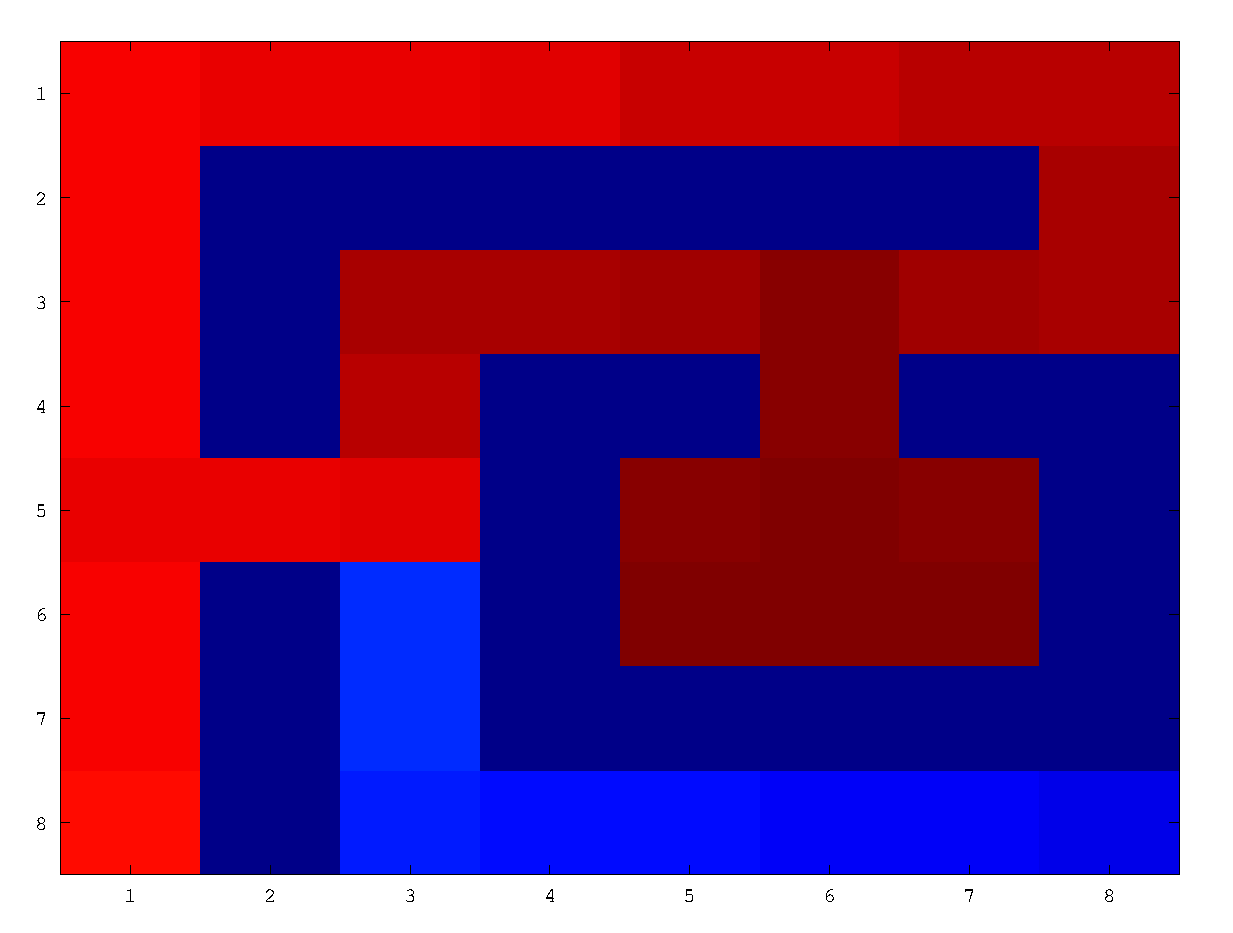
\includegraphics[width=0.45\textwidth]{../figures/pit_random_0_1}}
    \subfigure[$\omega = 0.5$]{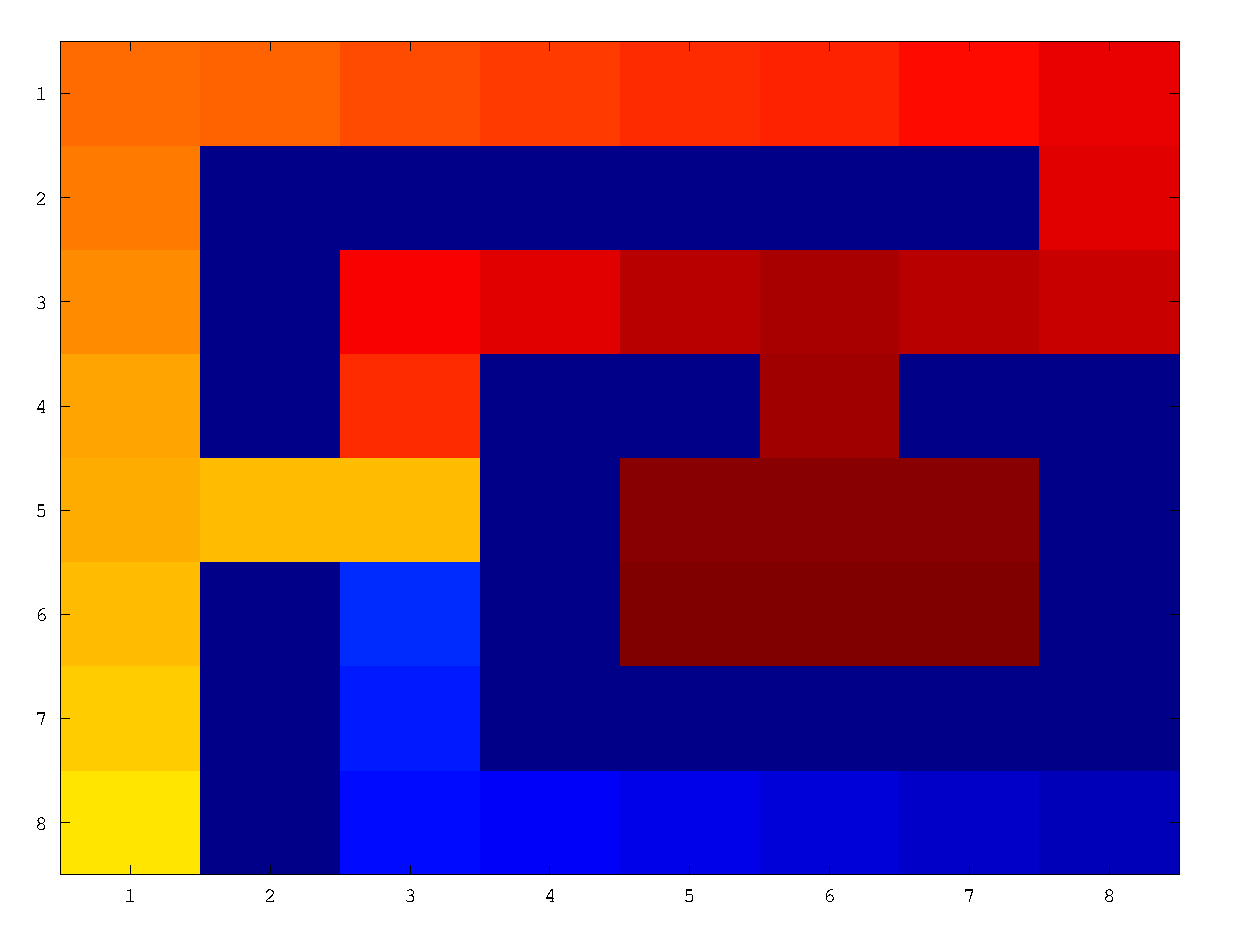
\includegraphics[width=0.45\textwidth]{../figures/pit_random_0_5}}
    \subfigure[value]{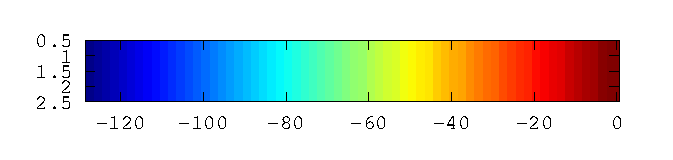
\includegraphics[width=0.45\textwidth]{../figures/color-axis}}
    \caption{Pit maze solutions for two values of $\omega$.}
    \label{fig:pit-solution}
  \end{figure}
Randomness changes the solution significantly in this environment. When $\omega$ is relatively small, it is worthwhile (in expectation) for the agent to pass past the pit, even though there is a risk of falling in and getting a reward of $-100$. In the example given, even starting from the third row, the agent prefers taking the short-cut. For high enough $\omega$, the optimal policy avoids approaching the pit. Still, the agent prefers jumping in the pit, than being trapped at the bottom of the maze forever.


\subsubsection{Continuing problems}
Finally, many problems have no natural terminating state, but are continuing \emph{ad infinitum}. Frequently, we model those problems using a utility that discounts future rewards exponentially. This way, we can guarantee that the utility is bounded. In addition, exponential discounting also has some economical sense. This is partially because of the effects of inflation, and partially because money now may be more useful than money in the future. Both these effects diminish the value of money over time.  As an example, consider the following inventory management problem. 

\begin{example}[Inventory management]
  There are $K$ storage locations, and each location $i$ can store
  $n_i$ items.  At each time-step there is a probability $\phi_i$ that
  a client tries to buy an item from location $i$, where $\sum_i
  \phi_i \leq 1$.  If there is an item available, when this happens,
  you gain reward $1$.  There are two types of actions, one for
  ordering a certain number $u$ units of stock, paying $c(u)$.
  Further one may move $u$ units of stock from one location $i$ to
  another location $j$, paying $\psi_{ij}(u)$.
\end{example}

An easy special case is when $K=1$, and we assume that deliveries
happen once every $m$ timesteps, and each time-step a client arrives
with probability $\phi$.  Then the state set $\CS=\{0, 1, \ldots, n
\}$ corresponds to the number of items we have, the action set
$\CA=\{0, 1, \ldots, n\}$ to the number of items we may order.  The
transition probabilities are given by $P(s'|s,a) =
\binom{m}{d}\phi^d(1-\phi)^{m-d}$, where $d=s+a-s'$, for $s+a \leq n$.
  % ro: What's the solution?
  % cd: I guess I should try and give the solution to this problem for these special cases.


\newcommand{\Node}[3]{%
  \pgfnodecircle{#1}[stroke]{#2}{0.3cm}%
  \pgfputat{\pgfrelative{#2}{\pgfxy(0,-.075)}}{\pgfbox[center,base]{#3}}}

\newcommand{\SNode}[3]{%
  \pgfnodebox{#1}[stroke]{#2}{0.3cm}%
  \pgfputat{\pgfrelative{#2}{\pgfxy(0,-.075)}}{\pgfbox[center,base]{#3}}}

\newcommand{\BNode}[3]{%
  \pgfnodecircle{#1}[stroke]{#2}{0.4cm}%
  \pgfputat{\pgfrelative{#2}{\pgfxy(0,-.075)}}{\pgfbox[center,base]{#3}}}

\newcommand{\Claim}[2]{%
  \pgfputat{\pgfrelative{\pgfxy(0.4,-0.075)}{\pgfnodecenter{#1}}}%
  {\pgfbox[left,base]{#2}}}

\newcommand{\LClaim}[2]{%
  \pgfputat{\pgfrelative{\pgfxy(-0.4,-0.075)}{\pgfnodecenter{#1}}}%
  {\pgfbox[right,base]{#2}}}

\newcommand{\Bush}[3]{%
  \pgfnodecircle{#1}[virtual]{\pgfrelative{\pgfnodecenter{#2}}{#3}}{1pt}%
  \pgfnodeconnline{#2}{#1}}



\subsection{MDP Algorithms}
\label{sec:mdp-algorithms}
\only<article>{Let us now look at three basic algorithms for solving a known Markov decision process. The first, \textit{value iteration}\index{value iteration}, is a simple extension of the backwards induction algorithm to the infinite horizon case. %This is possible to do, since the value converges and consequently we do not need to store all value vectors. %ro: outcommented this: also for backwards induction you need not store all the values, so didn't understand this
}
\subsubsection{Value iteration}
In this version of the algorithm, we assume that rewards are dependent only on the state. An algorithm for the case where reward only depends on the state can be obtained by replacing $r(s,a)$ with $r(s)$.
\label{sec:value-iteration}
\begin{frame}
  \begin{algorithm}[H]
    \begin{algorithmic}
      \State Input $\mdp$, $\CS$.
      \State Initialise $\val_0 \in \Vals$. %ro: What is \Vals here?
      \For{$n=1, 2, \ldots$}
      \For{$s \in \CS_n$}
      \State $\pol_n(s) = \argmax_{a \in \CA} \set{r(s, a) + \disc \sum_{s' \in \CS} P_\mdp(s' \mid s, a) \val_{n-1} (s')}$
      \State $\val_n(s) = r(s, \pol_n(s)) + \disc \sum_{s' \in \CS} P_\mdp(s' \mid s, \pol_n(s)) \val_{n-1} (s')$
      \EndFor
      \State \textbf{break} if \texttt{termination-condition} is met %ro: what is this condition?
      \EndFor
      \State Return $\pol_n, V_n$.
    \end{algorithmic}
    \caption{Value iteration}
  \end{algorithm}
\end{frame}

  The value iteration algortihm is a direct extension of the backwards induction algorithm for an infinite horizon. However, since we know that stationary policies are optimal, we do not need to maintain the values and actions for all time steps. At each step, we can merely keep the previous value $\val_{n-1}$. However, since there is an infinite number of steps, we need to know whether the algorithm converges to the optimal value, and what is the error we make at a particular iteration.
  \begin{theorem}
    The value iteration algorithm satisfies
    \begin{itemize}
    \item $\lim_{n \to \infty} \|\val_n - \val^*\| = 0$. 
    \item For each $\epsilon>0$ there exists $N_\epsilon <\infty$ such that for all $n\geq N_\epsilon$
      \begin{equation}
        \|\val_{n+1} - \val_n\| \leq \epsilon(1 - \disc)/2\disc.
        \label{eq:value-iteration-stopping}
      \end{equation}
    \item For $n\geq N_\epsilon$ the policy $\pol_\epsilon$ that takes action
      \[
      \argmax_a r(s,a) + \disc \sum_j p(j|s,a)\val_n(s')
      \]
      is
      $\epsilon$-optimal, i.e. $V^{\pol_\epsilon}_\mdp(s) \geq V^*_\mdp(s) - \epsilon$ for all states $s$.
    \item $\|\val_{n+1} - \val^*\| < \epsilon/2$ for $n \geq N_\epsilon$.
    \end{itemize}
  \end{theorem}
  \begin{proof}
    The first two statements follow from the fixed-point Theorem \ref{the:fixed-point}.
    Now note that
    \[
    \|V^{\pol_\epsilon}_\mdp - \val^*\|
    \leq
    \|V^{\pol_\epsilon}_\mdp - \val_n\|
    +
    \|\val_n - \val^*\|
    \]
    We can bound these two terms easily:  %ro: Some explanations would be helpful. Actually, I only understand the first equality. % cd: I had typos!
    \only<article>{
      \begin{align*}
        \norm{V^{\pol_\epsilon}_\mdp - \val_{n+1}}
        &= 
        \norm{\blm_{\pol_\epsilon} V^{\pol_\epsilon}_\mdp - \val_{n+1}}
        \tag{by definition of $\blm_{\pol_\epsilon}$}
        \\
        &\leq 
        \norm{\blm_{\pol_\epsilon} V^{\pol_\epsilon}_\mdp - \blm \val_{n+1}}
        +
        \norm{\blm \val_{n+1} - \val_{n+1}}
        \tag{triangle}
        \\
        &=
        \norm{\blm_{\pol_\epsilon} V^{\pol_\epsilon}_\mdp - \blm_{\pol_\epsilon} \val_{n+1}}
        +
        \norm{\blm \val_{n+1} - \blm \val_{n}}
        \tag{by definition}
        \\
        &\leq
        \disc \norm{V^{\pol_\epsilon}_\mdp - \val_{n+1}}
        +
        \disc \norm{\val_{n+1} -\val_{n}}.
        \tag{by contraction}
      \end{align*}
      An analogous argument gives the same bound for the second term  $\|\val_n - \val^*\|$. Then, rearranging we obtain
    }
    \[
    \norm{V^{\pol_\epsilon} - \val_{n+1}} 
    \leq
    \frac{\disc}{1 - \disc}\|\val_{n+1} - \val_{n}\|,
    \qquad
    \|\val_{n+1} - \val^*\|
    \leq
    \frac{\disc}{1 - \disc}\|\val_{n+1} - \val_{n}\|,
    \]
    and the third and fourth statements follow from the second statement.
  \end{proof}

  The \emindex{termination condition} of value iteration has been left unspecified. However, the theorem above shows that if we terminate when \eqref{eq:value-iteration-stopping} is true, then our error will be bounded by $\epsilon$. However, better termination conditions can be obtained.

Now let us prove how fast value iteration converges.
  \begin{theorem}[Value iteration monotonicity]
    Let $\Vals$ be the set of value vectors with Bellman operator $\blm$. Then:
    \begin{enumerate}
    \item Let $\val, \val' \in \Vals$ with $\val' \geq \val$. Then $\blm
      \val' \geq \blm \val$.
    \item Let $\val_{n+1} = \blm \val_n$. If there is an $N$ s.t.\ $\blm
      \val_N \leq \val_N$, then $\blm \val_{N+k} \leq \val_{N+k}$ for
      all $k \geq 0$ and similarly for $\geq$.
    \end{enumerate}
    \label{the:value-iteration-monotonicity}
  \end{theorem}
  \begin{proof}
    Let $\pol \in \argmax_\pol \vreward + \disc \trans_{\mdp,\pol} \val$. Then
    \[
    \blm \val
    = \vreward + \disc \trans_{\mdp,\pol} \val
    \leq \vreward + \disc \trans_{\mdp,\pol} \val'
    \leq \max_{\pol'}\vreward + \disc \trans_{\mdp,\pol'} \val',
    \]
    where the first inequality is due to the fact that $\trans \val \geq \trans \val'$ for any $\trans$.
    For the second part, 
    \[
    \blm \val_{N+k} = \val_{N+k+1} = \blm^k \blm \val_N \leq \blm^k \val_N = \val_{N+k}.
    \]
    since $\blm \val_N \leq \val_N$ by assumption and consequently $\blm^k \blm \val_N \leq \blm^k \val_N$ by part one of the theorem.
  \end{proof}

  Thus, value iteration converges monotonically to $V^*_{\mdp}$ if the
  initial value $\val_0 \leq \val'$ for all $\val'$.  If $r \geq 0$,
  it is sufficient to set $\val_0 = \mathbf{0}$. Then $\val_n$ is always
  a lower bound on the optimal value function.
\begin{theorem}
  Value iteration converges with error in $O(\disc^n)$
  More specifically, for $r \in [0,1]$ and $\val_0 = \mathbf{0}$, 
  \begin{align*}
    \|\val_n - V_\mdp^*\| &\leq \frac{\disc^n}{1 - \disc},
    &
    \|V^{\pol_n}_\mdp - V_\mdp^*\| &\leq \frac{2\disc^n}{1 - \disc}.
  \end{align*}
\end{theorem}
\begin{proof}
  The first part follows from the contraction property (Theorem~\ref{the:bellman-contraction}):
  \begin{equation}
    \|\val_{n+1} - \val^*\|
    =
    \|\blm \val_{n} - \blm \val^*\|
    \leq 
    \disc \|\val_{n} - \val^*\|.  %ro: This proves the convergence rate, what about the inequalities? 
  \end{equation}
  Now divide by $\disc^n$ to obtain the final result.
  
\end{proof}

Although value iteration converges exponentially fast, the convergence
is dominated by the discount factor $\disc$. When $\disc$ is very
close to one, convergence can be extremely slow.  In fact,
\citet{tseng1990solving} showed that the number of iterations are on
the order of $1 / (1 - \disc)$, for bounded accuracy of the input
data. The overall complexity is
$\tilde{O}(|\CS|^2 |\CA| L (1 - \disc)^{-1}$, omitting logarithmic
factors, where $L$ is the total number of bits used to represent the
input.\footnote{Thus the result is \emph{weakly} polynomial complexity, due to the dependence on the input size description.}
